\documentclass[11pt,a4paper]{article}

\usepackage[spanish,es-tabla]{babel}
\usepackage[utf8]{inputenc}
\usepackage[T1]{fontenc}
\usepackage{lmodern}
\usepackage[margin=2.2cm,top=2.5cm,bottom=2.5cm]{geometry}
\usepackage{amsmath,amssymb}
\usepackage{booktabs}
\usepackage{tabularx}
\usepackage{multirow}
\usepackage{graphicx}
\usepackage{xcolor}
\usepackage{hyperref}
\usepackage{caption}
\usepackage{subcaption}
\usepackage{enumitem}
\usepackage{fancyhdr}
\usepackage{microtype}
\usepackage{float}

% Paleta de colores Javeriana / IEEE
\definecolor{javnavy}{RGB}{16, 44, 87}
\definecolor{javblue}{RGB}{53, 95, 142}
\definecolor{tablehead}{RGB}{235, 240, 248}
\definecolor{tablerow}{RGB}{248, 250, 252}

\hypersetup{
    colorlinks=true,
    linkcolor=javnavy,
    citecolor=javblue,
    urlcolor=javblue
}

\pagestyle{fancy}
\fancyhf{}
\fancyhead[L]{\small\color{gray}Pontificia Universidad Javeriana · Tecnologías Emergentes}
\fancyhead[R]{\small\color{gray}Informe Final · San José del Palmar}
\fancyfoot[C]{\thepage}
\renewcommand{\headrulewidth}{0.4pt}

\captionsetup{font=small,labelfont={bf,color=javnavy},skip=6pt}

% ---------------------------------------------------------------------------
% ESTADO DE LA AUDITORIA RASTER: unico punto que se actualiza tras ejecutar
% src/audit_rasters_final.py sobre los GeoTIFF reales.
\newcommand{\estadoauditoria}{La correspondencia celda a celda entre los GeoTIFF de salida y estos conteos está pendiente de la auditoría con \texttt{src/audit\_rasters\_final.py}; las cifras provienen de los archivos \texttt{area\_stats\_*.json} generados por la inferencia oficial.}
\newcommand{\estadoauditoriacorto}{pendientes de auditoría directa sobre el GeoTIFF}
% ---------------------------------------------------------------------------

\title{\vspace{-1.2cm}
    \textbf{\Large Pontificia Universidad Javeriana}\\[0.2cm]
    \textbf{\large Departamento de Ingeniería de Sistemas — Tecnologías Emergentes}\\[0.6cm]
    \textbf{\LARGE Clasificación de Coberturas Terrestres Post-Sismo mediante Modelos de Machine Learning e Imágenes Sentinel-2 en San José del Palmar, Chocó}\\[0.3cm]
    \large Análisis comparativo de arquitecturas, optimización de hiperparámetros e inferencia geoespacial reproducible
}

\author{
    \textbf{Nicolás León} \quad \textbf{Andrés Felipe Barrios} \quad \textbf{Hania Valentina Carreño} \quad \textbf{Jorge Sierra}\\[0.2cm]
    \normalsize Profesor: Andrés Oswaldo Calderón Romero, Ph.D.\\[0.1cm]
    \small Bogotá D.C., Colombia · 26 de noviembre de 2026
}
\date{}

\begin{document}

\maketitle
\vspace{-0.6cm}

\begin{abstract}
\noindent Este informe documenta el desarrollo completo de un flujo de trabajo reproducible de Inteligencia Artificial Geoespacial (GeoAI) para discriminar y cartografiar cinco clases de cobertura terrestre en el municipio de San José del Palmar (Chocó, Colombia), en el cañón del río Ingará, afectado por el sismo de magnitud $M_w$~7,4 del 10 de agosto de 2026. A partir de una escena Sentinel-2 MSI Nivel-2A (reflectancia BOA) del 18 de agosto de 2026, se conformó un cubo multiespectral de diez bandas remuestreado a una grilla canónica de 10~m en el sistema de coordenadas oficial MAGNA-SIRGAS Origen Nacional (\texttt{EPSG:9377}). A partir de 145 polígonos de verdad de terreno con píxeles válidos, se estructuró un conjunto tabular de 14.155 píxeles etiquetados. Para disminuir el riesgo de fuga entre muestras del mismo polígono, la partición se realizó a nivel de \texttt{Polygon\_ID}, reservando 29 polígonos (2.708 píxeles) para prueba independiente y 116 polígonos (11.447 píxeles) en cuatro \textit{folds} espaciales de desarrollo. Sobre estos folds se optimizaron cinco arquitecturas mediante \texttt{GridSearchCV} con \texttt{scoring="f1\_macro"}: Regresión Logística (baseline), Árbol de Decisión (CART), Support Vector Machines (SVM con núcleo RBF), K-Nearest Neighbors (KNN) y una Red Neuronal Artificial (ANN / MLP). En el conjunto de prueba independiente ($N = 2.708$), SVM RBF alcanzó la mayor Exactitud Global (89,70~\%) y coeficiente Kappa (0,8283), mientras que la ANN/MLP logró el mayor Macro-F1 (0,7075 en test y 0,7103 en validación cruzada), métrica que pondera por igual las cinco clases; por ese criterio, definido antes de la evaluación, se seleccionó como modelo del mapa temático. En Urbano y Vías la precisión fue de 62,50~\% para ANN frente a 39,45~\% para SVM. Las importancias Gini del árbol destacaron \texttt{B08} (33,90~\%) y \texttt{B04} (32,58~\%), sin demostrar que cada banda sea indispensable. La inferencia se restringió a los 342.525 píxeles con datos válidos en las diez bandas (3.425,25~ha). Para ANN se registraron 2.189,51~ha de Bosque (63,92~\%), 1.172,13~ha de Suelo Desnudo y Roca (34,22~\%), 38,22~ha de Pastos y Cultivos (1,12~\%), 19,93~ha de Urbano y Vías (0,58~\%) y 5,46~ha de Agua (0,16~\%), \estadoauditoriacorto. Estos valores son predicciones espectrales de una sola escena posterior al evento y no demuestran por sí solos causalidad sísmica.
\end{abstract}

\vspace{0.3cm}
\noindent\textbf{Palabras clave:} GeoAI, Sentinel-2, MAGNA-SIRGAS, validación espacial agrupada, SVM, Red Neuronal Artificial, San José del Palmar, inferencia ráster.

\section{Introducción y contextualización del área de estudio}

El monitoreo ambiental mediante satélites ópticos de observación de la Tierra ha evolucionado desde clasificaciones manuales de escritorio hacia flujos de Inteligencia Artificial Geoespacial (GeoAI) desacoplados, programáticos y orientados a la reproducibilidad computacional. En regiones montañosas tropicales como la vertiente pacífica de la Cordillera Occidental colombiana, la alta nubosidad, la accidentada topografía y la dinámica de remoción en masa exigen metodologías rigurosas que impidan sobreestimar el rendimiento predictivo de los algoritmos.

El 10 de agosto de 2026 a las 12:34 UTC (7:34 a.~m. hora local), el Servicio Geológico Colombiano registró un evento sísmico de magnitud de momento $M_w$~7,4 a una profundidad intermedia de 103~km con epicentro en el municipio de San José del Palmar (Chocó)~\cite{sgc2026}. La escena posterior al evento permite estudiar coberturas relevantes para el seguimiento territorial, como suelo expuesto, vegetación y cauces. Sin comparación bitemporal ni validación externa adicional, la clasificación por sí sola no atribuye deslizamientos concretos al sismo.

Como insumo óptico se seleccionó una escena \textbf{Sentinel-2 MSI Nivel-2A} adquirida el 18 de agosto de 2026 (\texttt{S2C\_MSIL2A\_20260818T153621\_N0512\_R068\_T18NUL}), ocho días después del sismo, con reflectancia de superficie corregida atmosféricamente (\textit{Bottom-of-Atmosphere}, BOA). El objetivo del estudio es evaluar de forma rigurosa y comparativa cinco arquitecturas de aprendizaje automático supervisado para discriminar cinco categorías de cobertura: (1)~Bosque, (2)~Pastos y Cultivos, (3)~Suelo Desnudo y Roca, (4)~Urbano y Vías, y (5)~Agua, desplegando el clasificador seleccionado sobre toda la escena para cuantificar la superficie territorial post-evento en hectáreas y kilómetros cuadrados.

\subsection{Zona de estudio, metadatos de la escena y verdad de terreno}
La Tabla~\ref{tab:metadatos} resume los datos de entrada de la Fase~1. La región de interés (ROI) es un polígono de 4.921,30~ha sobre el cañón del río Ingará (\texttt{data/vectors/roi\_palmar.geojson}). La grilla de trabajo cubre 7.177,74~ha; dentro de ella, la máscara de calidad (\texttt{mask\_valid.tif}) habilita 471.579 celdas.

\begin{table}[H]
\centering
\small
\begin{tabularx}{\textwidth}{l X}
\toprule
\textbf{Atributo} & \textbf{Valor} \\
\midrule
Evento de referencia & Sismo $M_w$~7,4, 10/08/2026, 12:34~UTC, profundidad 103~km (SGC)~\cite{sgc2026} \\
Producto & \texttt{S2C\_MSIL2A\_20260818T153621\_N0512\_R068\_T18NUL} \\
Sensor / nivel & Sentinel-2C MSI, Nivel-2A (reflectancia de superficie BOA) \\
Adquisición & 18/08/2026, 15:36:21~UTC (órbita relativa R068, tesela T18NUL, línea base N0512) \\
ROI (WGS84) & Longitud $-76{,}3095^\circ$ a $-76{,}2147^\circ$; latitud $4{,}8699^\circ$ a $4{,}9312^\circ$ \\
CRS de trabajo & MAGNA-SIRGAS Origen Nacional (\texttt{EPSG:9377}); CRS nativo WGS~84 / UTM~18N (\texttt{EPSG:32618}) \\
Grilla & $1.054 \times 681$ píxeles de $10 \times 10$~m (717.774 celdas) \\
Bandas & 10: \texttt{B02}, \texttt{B03}, \texttt{B04}, \texttt{B05}, \texttt{B06}, \texttt{B07}, \texttt{B08}, \texttt{B8A}, \texttt{B11}, \texttt{B12} \\
Verdad de terreno & 240 polígonos digitalizados en \texttt{data/vectors/ground\_truth.gpkg}; 145 aportaron píxeles válidos al TSV \\
\bottomrule
\end{tabularx}
\caption{Metadatos de la escena, de la región de estudio y de la verdad de terreno (Fase~1).}
\label{tab:metadatos}
\end{table}

Los 95 polígonos sin muestras se encuentran dentro de la ROI y tienen un tamaño mediano similar al de los incluidos (0,30~ha frente a 0,34~ha). La explicación documentada es que sus píxeles quedan en zonas sin datos válidos de la escena; la verificación individual por polígono contra el stack y la máscara se reporta como pendiente en la Sección~\ref{sec:limitaciones}.

\section{Preparación del cubo multiespectral y extracción tabular}

\subsection{Sistema canónico de referencia espacial y grilla canónica}
Para evitar distorsiones métricas y asegurar compatibilidad con la cartografía oficial del Instituto Geográfico Agustín Codazzi (IGAC), todas las capas fueron reproyectadas al sistema canónico nacional \textbf{MAGNA-SIRGAS Origen Nacional (\texttt{EPSG:9377})}. Se consolidó una grilla canónica de $1.054 \times 681$ píxeles a una resolución espacial de $10\text{ m} \times 10\text{ m}$ por celda ($100\text{ m}^2 = 0,01\text{ ha}$), preservando la matriz de transformación afín oficial.

\subsection{Stack multiespectral de 10 bandas}
El cubo ráster consolidado (\texttt{data/processed/stack\_10bands.tif}) reúne diez bandas espectrales del instrumento MSI~\cite{lillesand2015}. Las bandas nativas de 20~m fueron remuestreadas a la resolución común de 10~m mediante interpolación bilineal (Tabla~\ref{tab:bandas}):

\begin{table}[H]
\centering
\small
\begin{tabularx}{\textwidth}{c c l c c c X}
\toprule
\textbf{Índice} & \textbf{Banda} & \textbf{Región espectral} & $\boldsymbol{\lambda_c}$ \textbf{(nm)} & \textbf{Res. Nativa} & \textbf{Grilla} & \textbf{Función biofísica principal} \\
\midrule
1 & \texttt{B02} & Azul visible & 490 & 10 m & 10 m & Penetración en agua, dispersión Rayleigh residual y reflectancia urbana. \\
2 & \texttt{B03} & Verde visible & 560 & 10 m & 10 m & Pico de reflectancia foliar de la vegetación y turbidez en cuerpos de agua. \\
3 & \texttt{B04} & Rojo visible & 665 & 10 m & 10 m & Fuerte absorción por clorofila; contraste directo suelo desnudo vs. vegetación. \\
4 & \texttt{B05} & Red Edge 1 & 705 & 20 m & 10 m & Pendiente del borde rojo; discriminación de biomasa foliar y estrés. \\
5 & \texttt{B06} & Red Edge 2 & 740 & 20 m & 10 m & Transición estructural foliar; separación dosel arbóreo denso vs. pastos. \\
6 & \texttt{B07} & Red Edge 3 & 783 & 20 m & 10 m & Hombro superior del infrarrojo; contenido celular y densidad de follaje. \\
7 & \texttt{B08} & NIR amplio & 842 & 10 m & 10 m & Meseta infrarroja de alta dispersión en mesófilo y fuerte absorción en agua. \\
8 & \texttt{B8A} & NIR estrecho & 865 & 20 m & 10 m & Banda espectral angosta libre de absorción de vapor de agua. \\
9 & \texttt{B11} & SWIR 1 & 1610 & 20 m & 10 m & Contenido hídrico foliar y del suelo; alta respuesta en roca y cicatrices secas. \\
10 & \texttt{B12} & SWIR 2 & 2190 & 20 m & 10 m & Caracterización mineralógica (arcillas/óxidos) y superficies construidas. \\
\bottomrule
\end{tabularx}
\caption{Características físicas y especificación espectral de las diez bandas Sentinel-2 empleadas en el estudio.}
\label{tab:bandas}
\end{table}

\subsection{Extracción y estructura del archivo tabular TSV}
A través del módulo \texttt{src/02\_extract\_tsv.py}, se intersectaron los polígonos de verdad de terreno (\texttt{data/training/ground\_truth.gpkg}) con \texttt{stack\_10bands.tif}. Se aplicó el criterio geométrico \texttt{all\_touched=False} (centro del píxel contenido en el polígono) y reintento con \texttt{all\_touched=True} únicamente para polígonos lineales estrechos. Se descartaron valores nulos, infinitos y reflectancias físicas fuera de $[0, 1]$.

El archivo resultante \texttt{data/training/dataset.tsv} (SHA-256: \texttt{f90bc6588...}) contiene 14.155 registros estructurados en 15 columnas:
\begin{enumerate}[noitemsep,topsep=2pt]
    \item \textbf{Variables predictoras (matriz $\boldsymbol{X}$):} Las diez reflectancias espectrales (\texttt{B02}, \texttt{B03}, \texttt{B04}, \texttt{B05}, \texttt{B06}, \texttt{B07}, \texttt{B08}, \texttt{B8A}, \texttt{B11}, \texttt{B12}). No se incorporan coordenadas en el entrenamiento para evitar que los modelos sobreajusten memorizando posiciones espaciales.
    \item \textbf{Variables de agrupación y respuesta:} \texttt{Polygon\_ID} (clave de partición espacial), \texttt{Class\_ID} (código numérico 1 a 5) y \texttt{Class} (etiqueta categórica).
    \item \textbf{Trazabilidad geográfica:} \texttt{Latitude} y \texttt{Longitude} (WGS84).
\end{enumerate}

\begin{table}[H]
\centering
\small
\begin{tabular}{l l c c c c c}
\toprule
\textbf{Polygon\_ID} & \textbf{Clase real (\texttt{Class})} & \textbf{B02} & \textbf{B04} & \textbf{B08} & \textbf{B11} & \textbf{B12} \\
\midrule
\texttt{poly\_sue\_001} & Suelo Desnudo y Roca & 0,03066 & 0,05546 & 0,30171 & 0,21701 & 0,10591 \\
\texttt{poly\_bos\_001} & Bosque               & 0,02410 & 0,02450 & 0,43349 & 0,21077 & 0,08741 \\
\texttt{poly\_pas\_001} & Pastos y Cultivos    & 0,03888 & 0,05409 & 0,27997 & 0,21045 & 0,10816 \\
\texttt{poly\_urb\_002} & Urbano y Vías        & 0,08691 & 0,09114 & 0,16153 & 0,22448 & 0,20800 \\
\texttt{poly\_agu\_001} & Agua                 & 0,05982 & 0,08268 & 0,10294 & 0,11185 & 0,07525 \\
\bottomrule
\end{tabular}
\caption{Registros representativos del archivo \texttt{data/training/dataset.tsv} (subconjunto de cinco bandas).}
\label{tab:tsv_sample}
\end{table}

\section{Metodología de validación espacial y modelado}

\subsection{Estrategia de partición espacial agrupada por polígono}
La autocorrelación espacial inherente a las imágenes de satélite invalida el uso del remuestreo aleatorio tradicional (\textit{random k-fold} o \textit{train\_test\_split} por fila): píxeles contiguos pertenecientes a una misma masa forestal o cicatriz comparten reflectancias casi idénticas. Mezclarlos entre entrenamiento y prueba produce una sobreestimación artificial del desempeño al evaluar píxeles prácticamente memorizados.

Para reducir este sesgo, la unidad de separación en \texttt{src/spatial\_split.py} es el \texttt{Polygon\_ID}:
\begin{itemize}[noitemsep,topsep=2pt]
    \item \textbf{Conjunto de desarrollo (Dev):} 116 polígonos con 11.447 píxeles (80,87~\% del dataset), organizados en 4 folds espaciales estratificados para ajuste y búsqueda de hiperparámetros.
    \item \textbf{Conjunto de prueba independiente (Test):} 29 polígonos con 2.708 píxeles (19,13~\% del dataset). Ningún píxel de estos polígonos intervino directa ni indirectamente en el entrenamiento ni en la optimización.
\end{itemize}
Las particiones oficiales se registraron en \texttt{data/training/spatial\_partitions.json} con semilla fija 42. Se comprobó que ningún polígono aparece a la vez en desarrollo y prueba. La partición por polígono evita compartir píxeles de un mismo polígono entre conjuntos, aunque no elimina necesariamente la autocorrelación entre polígonos vecinos~\cite{roberts2017}. El conjunto de prueba contiene 3 polígonos de Bosque, 2 de Pastos y Cultivos, 22 de Suelo Desnudo y Roca, 1 de Urbano y Vías y 1 de Agua; por ello, las métricas de las clases minoritarias dependen de muy pocos polígonos independientes.

\begin{table}[H]
\centering
\small
\resizebox{\textwidth}{!}{\begin{tabular}{c l c c c c c}
\toprule
\textbf{Class\_ID} & \textbf{Cobertura terrestre} & \textbf{Polígonos} & \textbf{Píxeles Dev} & \textbf{Píxeles Test} & \textbf{Total píxeles} & \textbf{Proporción (\%)} \\
\midrule
1 & Bosque                  & 13  & 6.194  & 1.222 & 7.416  & 52,39\,\% \\
3 & Suelo Desnudo y Roca    & 108 & 3.679  & 1.189 & 4.868  & 34,39\,\% \\
4 & Urbano y Vías           & 6   & 800    & 71    & 871    & 6,15\,\%  \\
2 & Pastos y Cultivos       & 12  & 636    & 203   & 839    & 5,93\,\%  \\
5 & Agua                    & 6   & 138    & 23    & 161    & 1,14\,\%  \\
\midrule
— & \textbf{Total}          & \textbf{145} & \textbf{11.447} & \textbf{2.708} & \textbf{14.155} & \textbf{100,00\,\%} \\
\bottomrule
\end{tabular}}
\caption{Distribución por clase y partición espacial en \texttt{dataset.tsv}.}
\label{tab:clases_particion}
\end{table}

\subsection{Implementación y optimización de hiperparámetros (HPO)}
Cada arquitectura se empaquetó en un \texttt{Pipeline} de Scikit-Learn~\cite{pedregosa2011} incorporando estandarización (\texttt{StandardScaler}) en los modelos sensibles a escala (LR, SVM, KNN, ANN). La optimización se realizó con \texttt{GridSearchCV} sobre los 4 folds de desarrollo con la métrica \textbf{Macro-F1}, que pondera por igual las cinco clases y por ello es menos sensible al desbalance que la exactitud global. Las grillas, definidas en \texttt{config/project.yaml}, suman 50 combinaciones (LR~6, Árbol~24, SVM~6, KNN~8, ANN~6), cada una evaluada en los 4 folds:
\begin{enumerate}[noitemsep,topsep=2pt]
    \item \textbf{Regresión Logística (Baseline obligatorio):} Modelo lineal multiclase con penalización $L_2$. Mejor configuración: $C = 1,0$, \texttt{class\_weight='balanced'}, \texttt{max\_iter=1000}.
    \item \textbf{Árbol de Decisión (CART):} Modelo jerárquico ortogonal por impureza de Gini. Mejor configuración: \texttt{max\_depth=8}, \texttt{min\_samples\_leaf=2}, \texttt{class\_weight='balanced'}.
    \item \textbf{Support Vector Machines (SVM RBF):} Hiperplano óptimo no lineal en espacio de Hilbert. Mejor configuración: núcleo RBF, $C = 10,0$, $\gamma = \text{'scale'}$.
    \item \textbf{K-Nearest Neighbors (KNN):} Clasificación basada en vecindad espectral ponderada. Mejor configuración: $k = 15$, ponderación inversa a la distancia (\texttt{weights='distance'}).
    \item \textbf{Red Neuronal Artificial (ANN / MLP):} Perceptrón multicapa feedforward con regularización $L_2$ ($\alpha$) y optimizador Adam. Mejor configuración: dos capas ocultas $(64, 32)$, $\alpha = 0,0001$, \texttt{max\_iter=500}.
\end{enumerate}

\subsection{Importancia espectral de bandas en el Árbol de Decisión}
En correspondencia con la Sección 3.2 del enunciado, la extracción de la importancia por reducción de impureza de Gini en \texttt{models/decision\_tree.joblib} permite identificar cuáles regiones espectrales definen los cortes óptimos de clasificación (Figura~\ref{fig:importancia} y Tabla~\ref{tab:importancia}):

\begin{figure}[H]
    \centering
    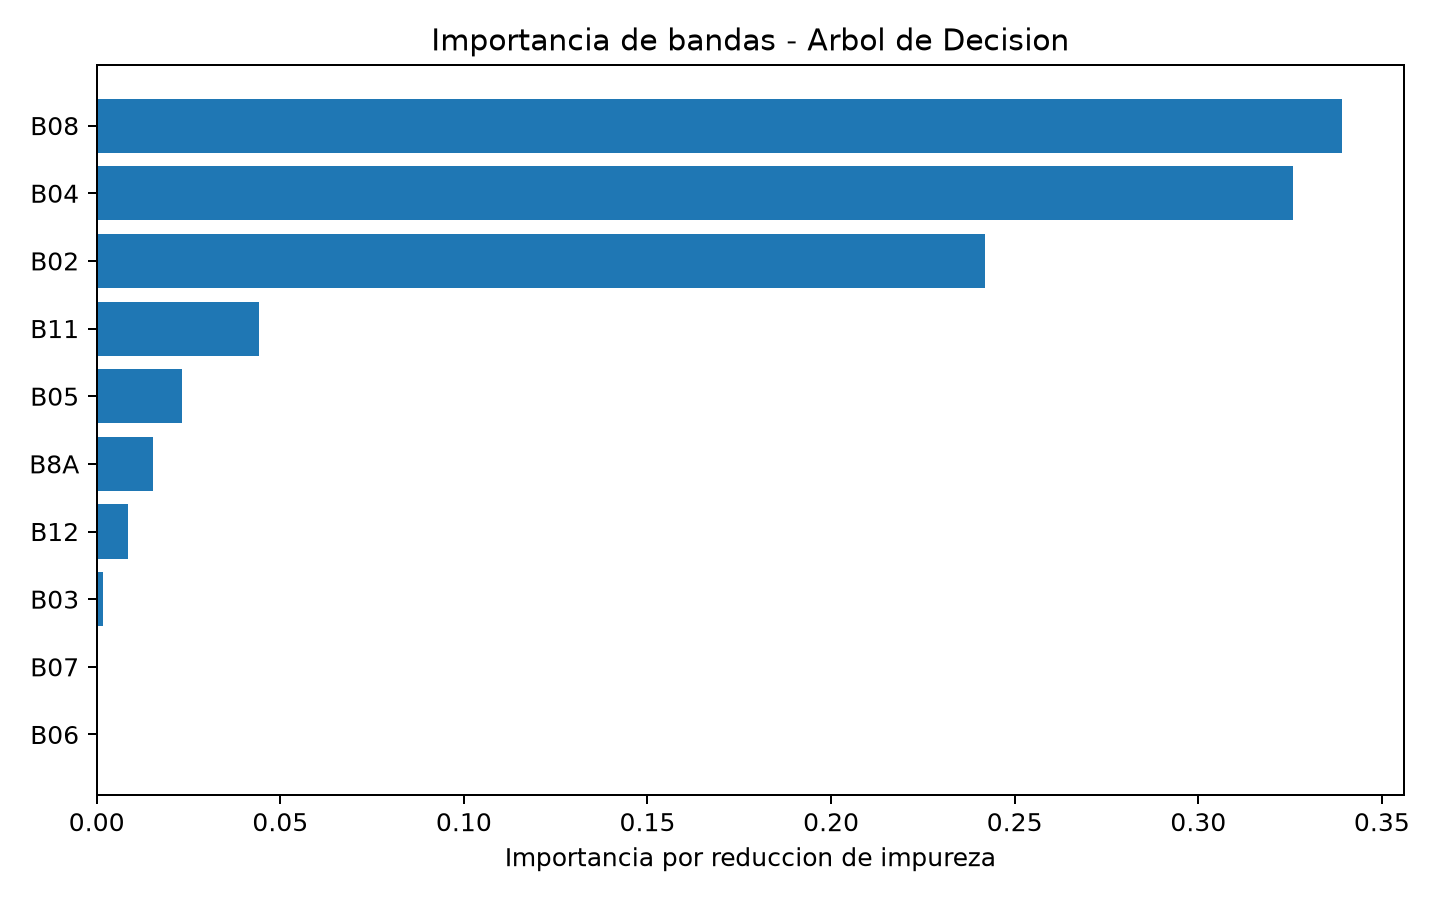
\includegraphics[width=0.78\textwidth]{figures/decision_tree_band_importance.png}
    \caption{Importancia relativa de las bandas Sentinel-2 en el Árbol de Decisión óptimo (\texttt{max\_depth=8}).}
    \label{fig:importancia}
\end{figure}

\begin{table}[H]
\centering
\small
\begin{tabularx}{\textwidth}{c l l c r X}
\toprule
\textbf{Rango} & \textbf{Banda} & \textbf{Región espectral} & $\boldsymbol{\lambda_c}$ \textbf{(nm)} & \textbf{Importancia (\%)} & \textbf{Interpretación en el paisaje montañoso} \\
\midrule
1 & \texttt{B08} & NIR amplio & 842 & \textbf{33,90\,\%} & Separación fotosintética de vegetación sana vs. suelo mineral y agua. \\
2 & \texttt{B04} & Rojo visible & 665 & \textbf{32,58\,\%} & Absorción clorofílica; junto con \texttt{B08} reproduce el contraste del NDVI. \\
3 & \texttt{B02} & Azul visible & 490 & \textbf{24,18\,\%} & Detección de cuerpos de agua y superficies urbanas/teñidas de alta reflectancia. \\
4 & \texttt{B11} & SWIR 1 & 1610 & \textbf{4,42\,\%} & Discriminación de humedad edáfica y mineralogía en roca y cicatrices. \\
5 & \texttt{B05} & Red Edge 1 & 705 & \textbf{2,31\,\%} & Umbrales de transición entre bosque denso y vegetación secundaria/pastos. \\
6 & \texttt{B8A} & NIR estrecho & 865 & \textbf{1,54\,\%} & Estabilización infrarroja en laderas con contraste de sombra. \\
7 & \texttt{B12} & SWIR 2 & 2190 & \textbf{0,86\,\%} & Respuestas arcillosas en taludes expuestos y vialidad. \\
8--10 & \texttt{B03, B07, B06} & Verde / RE 2--3 & — & \textbf{0,20\,\%} & Información colineal absorbida por los cortes superiores en \texttt{B08} y \texttt{B04}. \\
\bottomrule
\end{tabularx}
\caption{Desglose de importancia de bandas espectrales del Árbol de Decisión.}
\label{tab:importancia}
\end{table}

Las bandas \texttt{B08} (33,90~\%) y \texttt{B04} (32,58~\%) concentran el \textbf{66,48~\%} de la importancia Gini del árbol entrenado. \texttt{B02} (24,18~\%), \texttt{B11} (4,42~\%) y \texttt{B05} (2,31~\%) también aportan a sus decisiones. Estas cifras describen el uso de las bandas en este estimador, pero no prueban que cada banda sea indispensable; eso exigiría un experimento de eliminación de características.

\section{Resultados comparativos y evaluación en el test independiente}

\subsection{Tabla maestra comparativa de las cinco arquitecturas}
La Tabla~\ref{tab:comparacion_modelos} resume el desempeño global sobre las 2.708 muestras de prueba independientes ($N = 2.708$), reportando Exactitud Global, coeficiente Kappa de Cohen~\cite{congalton2019}, Macro-F1, Weighted-F1, el promedio obtenido en validación cruzada sobre desarrollo y el tiempo de optimización:

\begin{table}[H]
\centering
\small
\resizebox{\textwidth}{!}{\begin{tabular}{l c c c c c r}
\toprule
\textbf{Modelo} & \textbf{Overall Accuracy} & \textbf{Kappa ($\boldsymbol{\kappa}$)} & \textbf{Macro-F1 (Test)} & \textbf{Weighted-F1} & \textbf{CV Macro-F1 (Dev)} & \textbf{Tiempo HPO} \\
\midrule
\textbf{ANN / MLP} \texttt{(64, 32)} & 88,74\,\% (2.403/2.708) & 0,8146 & \textbf{0,7075} & 0,8929 & \textbf{0,7103 $\pm$ 0,0866} & 103,64 s \\
\textbf{SVM (RBF)} $C=10$            & \textbf{89,70\,\%} (2.429/2.708) & \textbf{0,8283} & 0,6889 & \textbf{0,8965} & 0,6538 $\pm$ 0,0830 & 7,32 s \\
\textbf{Árbol de Decisión} $d=8$     & 86,41\,\% (2.340/2.708) & 0,7827 & 0,6794 & 0,8795 & 0,6926 $\pm$ 0,0923 & 7,51 s \\
\textbf{Reg. Logística} (Baseline)   & 82,87\,\% (2.244/2.708) & 0,7343 & 0,6516 & 0,8505 & 0,7039 $\pm$ 0,0749 & 5,81 s \\
\textbf{KNN} ($k=15$, distance)      & 87,70\,\% (2.375/2.708) & 0,7936 & 0,6159 & 0,8708 & 0,6805 $\pm$ 0,0961 & 4,17 s \\
\bottomrule
\end{tabular}}
\caption{Comparación estadística general de las cinco arquitecturas evaluadas en el conjunto de prueba independiente.}
\label{tab:comparacion_modelos}
\end{table}

\subsection{Evaluación detallada por clase: Precisión, Exhaustividad (Recall) y F1-Score}
En cumplimiento explícito de la Sección 3.3 del enunciado, la Tabla~\ref{tab:metricas_clase} detalla la confiabilidad (\textit{Precision}), completitud (\textit{Recall}) y media armónica (\textit{F1-Score}) para cada una de las cinco coberturas en el test reservado:

\begin{table}[H]
\centering
\small
\resizebox{\textwidth}{!}{\begin{tabular}{l c c c c c c}
\toprule
\textbf{Clase (Soporte Test)} & \textbf{Métrica} & \textbf{Reg. Logística} & \textbf{Árbol Decisión} & \textbf{SVM (RBF)} & \textbf{KNN ($\boldsymbol{k=15}$)} & \textbf{ANN / MLP} \\
\midrule
\multirow{3}{*}{\textbf{Agua} ($n = 23$)} 
& Precision & 0,4510 & 0,4510 & \textbf{0,4792} & 0,4694 & \textbf{0,4792} \\
& Recall    & \textbf{1,0000} & \textbf{1,0000} & \textbf{1,0000} & \textbf{1,0000} & \textbf{1,0000} \\
& F1-Score  & 0,6216 & 0,6216 & \textbf{0,6479} & 0,6389 & \textbf{0,6479} \\
\midrule
\multirow{3}{*}{\textbf{Bosque} ($n = 1.222$)} 
& Precision & 0,9984 & \textbf{1,0000} & 0,9992 & 0,9992 & 0,9992 \\
& Recall    & \textbf{1,0000} & \textbf{1,0000} & \textbf{1,0000} & \textbf{1,0000} & \textbf{1,0000} \\
& F1-Score  & 0,9992 & \textbf{1,0000} & 0,9996 & 0,9996 & 0,9996 \\
\midrule
\multirow{3}{*}{\textbf{Pastos y Cultivos} ($n = 203$)} 
& Precision & 0,3251 & 0,3239 & \textbf{0,4868} & 0,3793 & 0,3658 \\
& Recall    & \textbf{0,7094} & 0,5665 & 0,3645 & 0,1626 & 0,4631 \\
& F1-Score  & \textbf{0,4458} & 0,4122 & 0,4169 & 0,2276 & 0,4087 \\
\midrule
\multirow{3}{*}{\textbf{Suelo Desnudo / Roca} ($n = 1.189$)} 
& Precision & \textbf{0,9599} & 0,9514 & 0,9073 & 0,8763 & 0,9176 \\
& Recall    & 0,6838 & 0,7897 & \textbf{0,8974} & 0,8940 & 0,8612 \\
& F1-Score  & 0,7986 & 0,8631 & \textbf{0,9023} & 0,8851 & 0,8885 \\
\midrule
\multirow{3}{*}{\textbf{Urbano y Vías} ($n = 71$)} 
& Precision & 0,2937 & 0,4409 & 0,3945 & 0,2500 & \textbf{0,6250} \\
& Recall    & 0,5915 & 0,5775 & \textbf{0,6056} & 0,4789 & 0,5634 \\
& F1-Score  & 0,3925 & 0,5000 & 0,4778 & 0,3285 & \textbf{0,5926} \\
\bottomrule
\end{tabular}}
\caption{Precisión, Exhaustividad (Recall) y F1-Score por cobertura en el test independiente ($N = 2.708$).}
\label{tab:metricas_clase}
\end{table}

\subsection{Análisis comparativo de las matrices de confusión}
Las matrices de confusión (orden: Agua, Bosque, Pastos, Suelo, Urbano) evidencian patrones de error distintivos entre familias algorítmicas:

\begin{figure}[H]
    \centering
    \begin{subfigure}[b]{0.48\textwidth}
        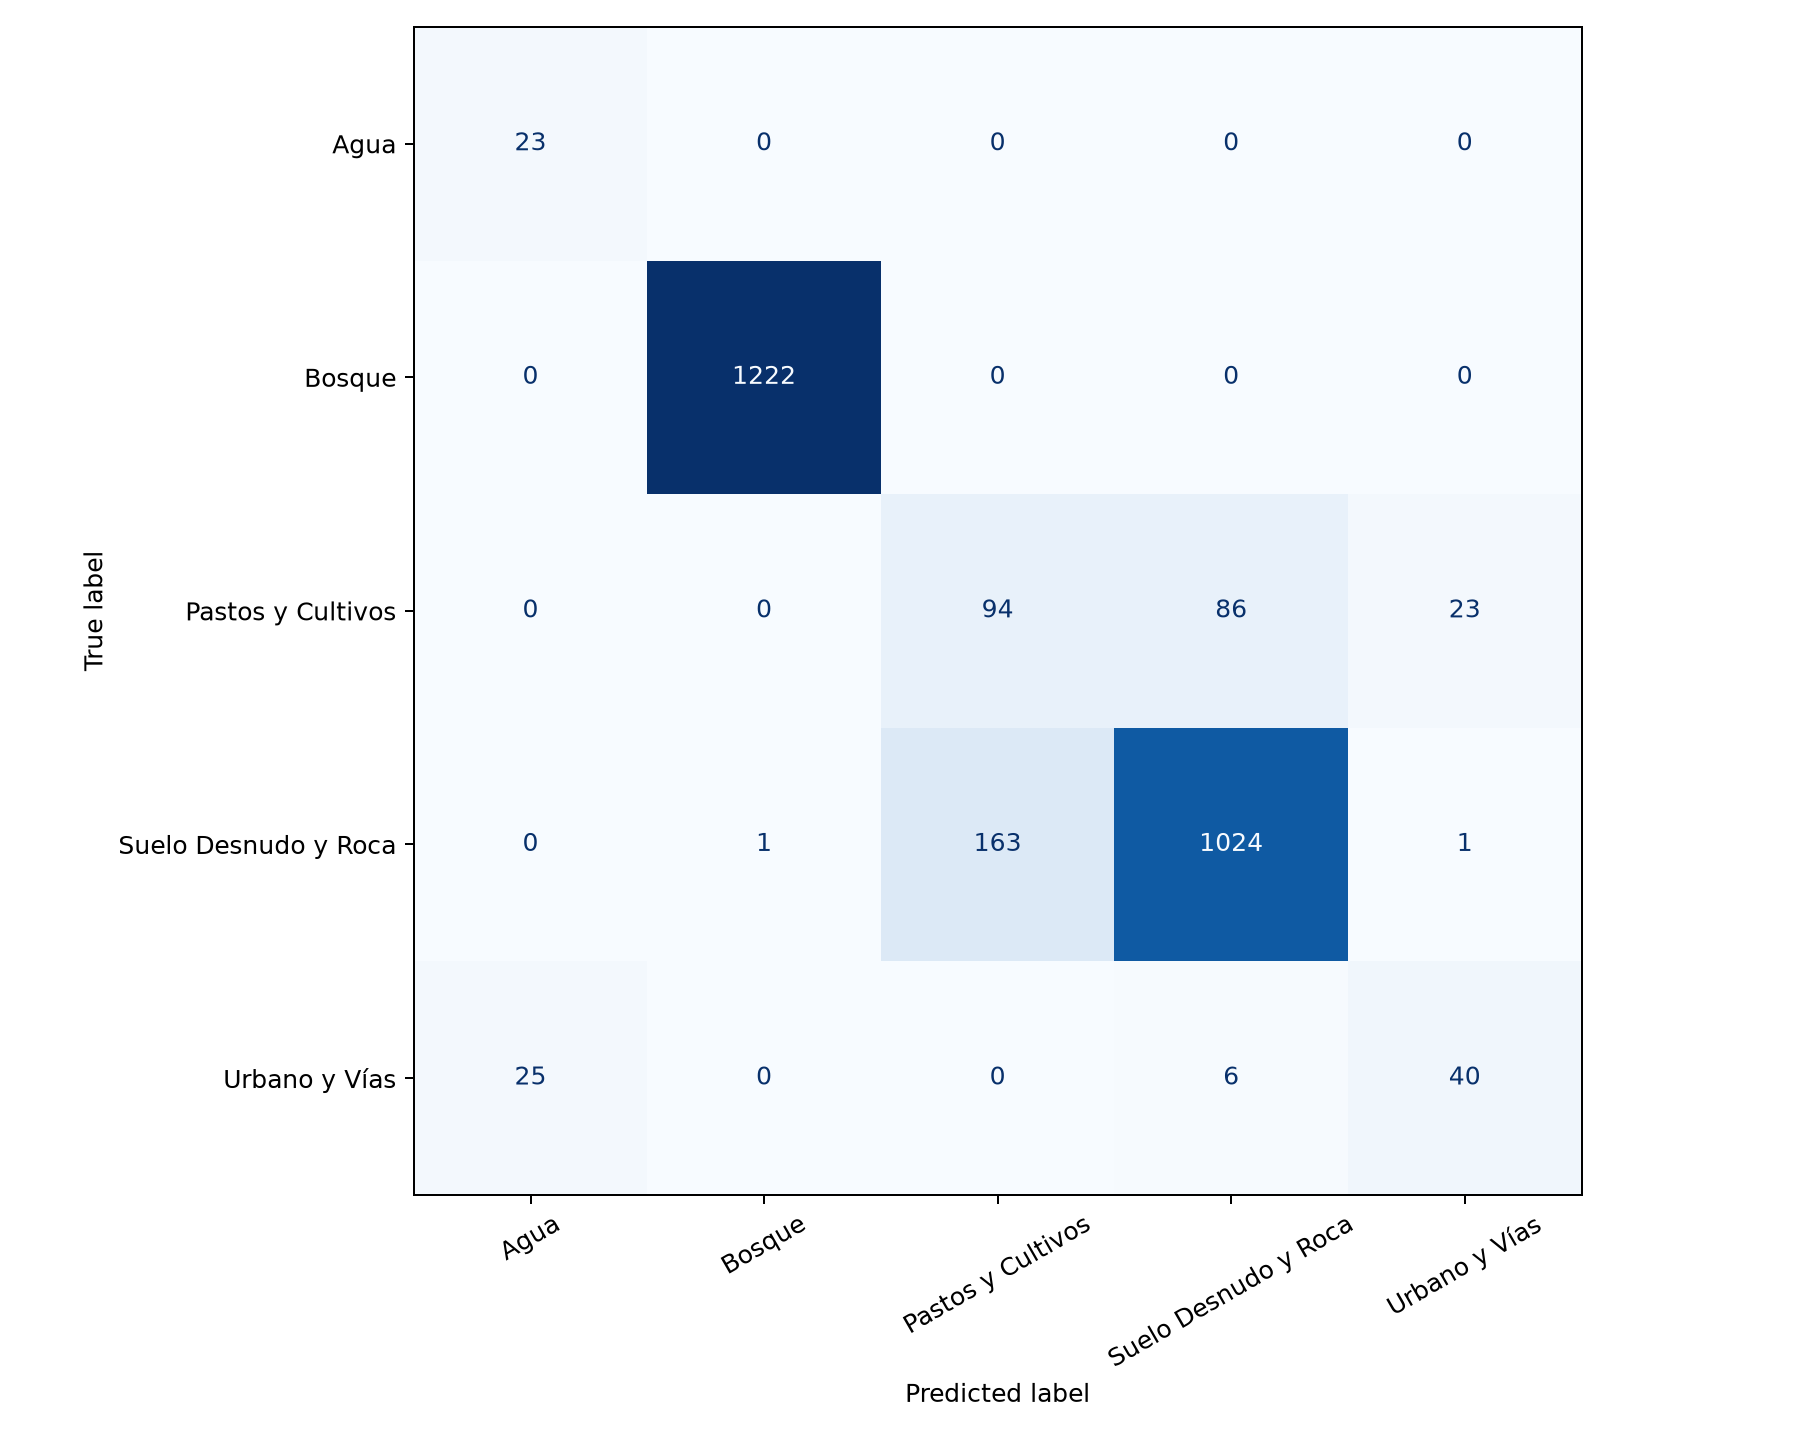
\includegraphics[width=\textwidth]{figures/ann_confusion_matrix.png}
        \caption{Red Neuronal Artificial (ANN/MLP): 2.403/2.708.}
    \end{subfigure}
    \hfill
    \begin{subfigure}[b]{0.48\textwidth}
        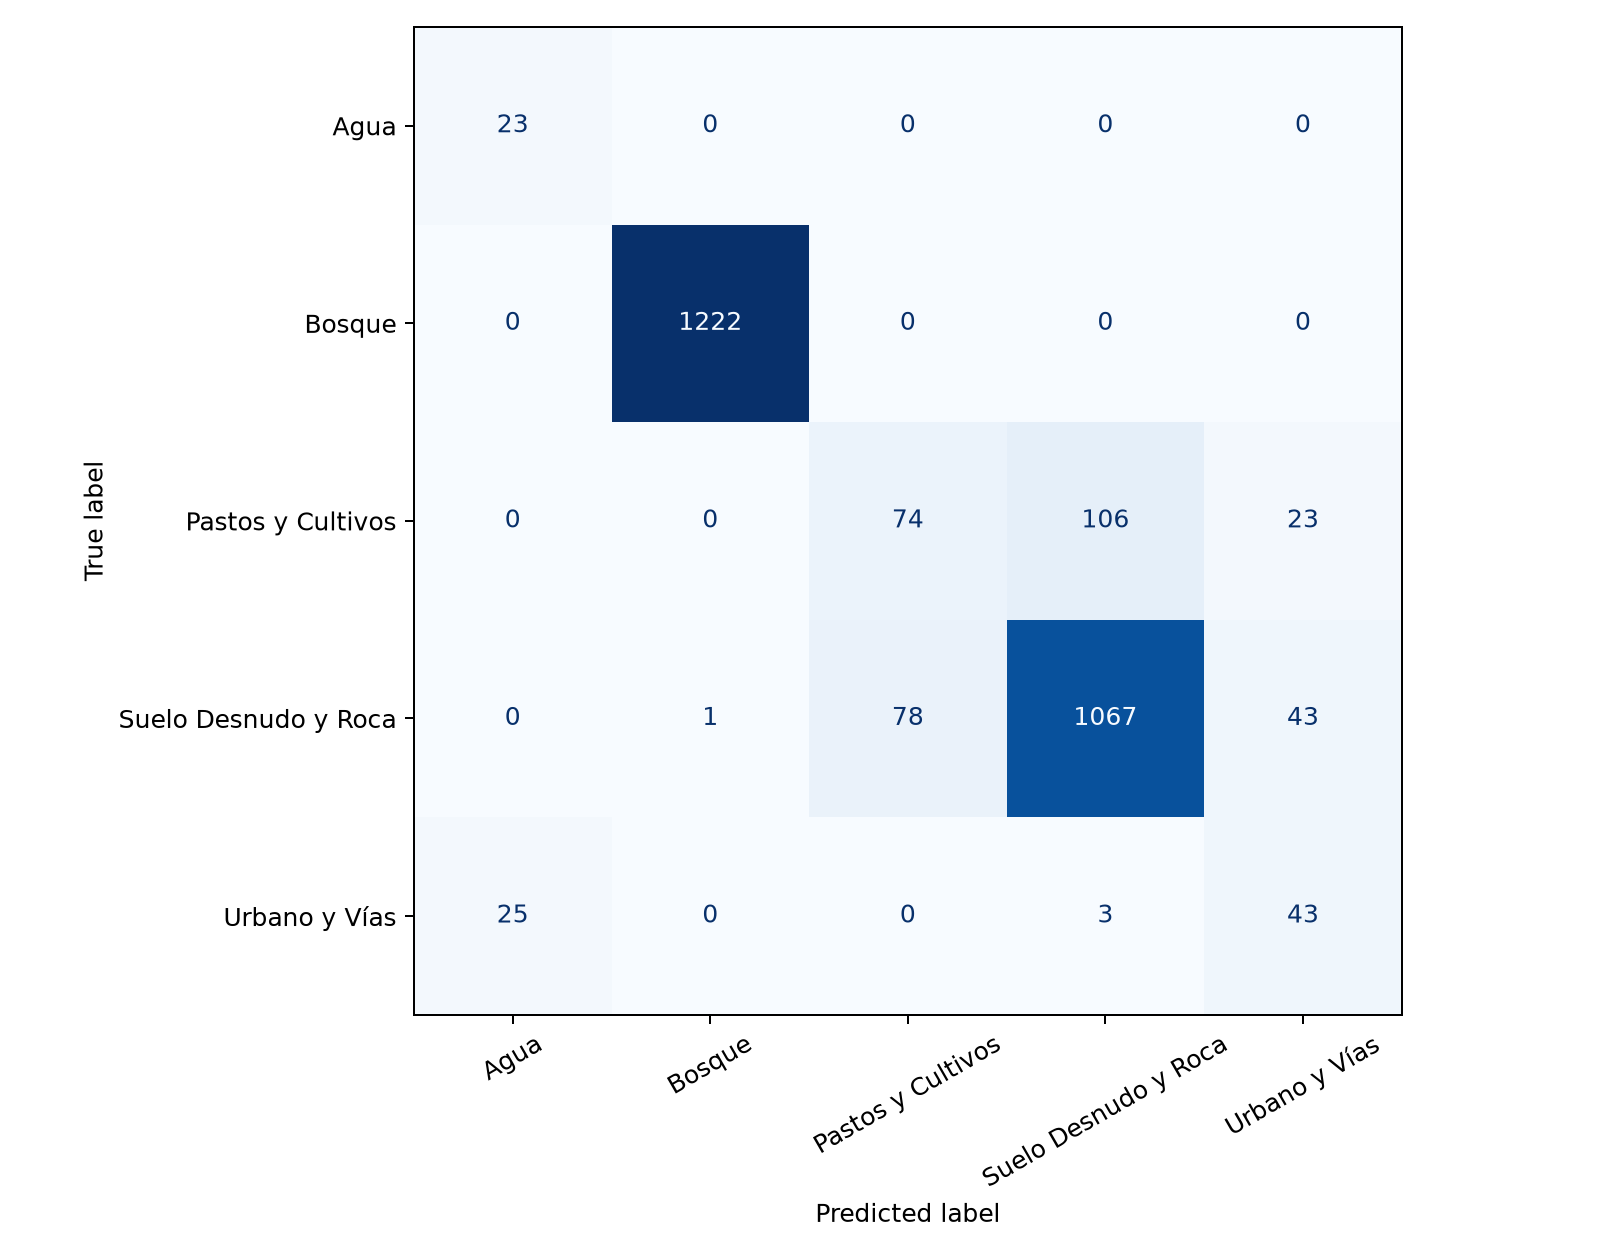
\includegraphics[width=\textwidth]{figures/svm_confusion_matrix.png}
        \caption{SVM con núcleo RBF: 2.429/2.708.}
    \end{subfigure}\\[0.3cm]
    \begin{subfigure}[b]{0.48\textwidth}
        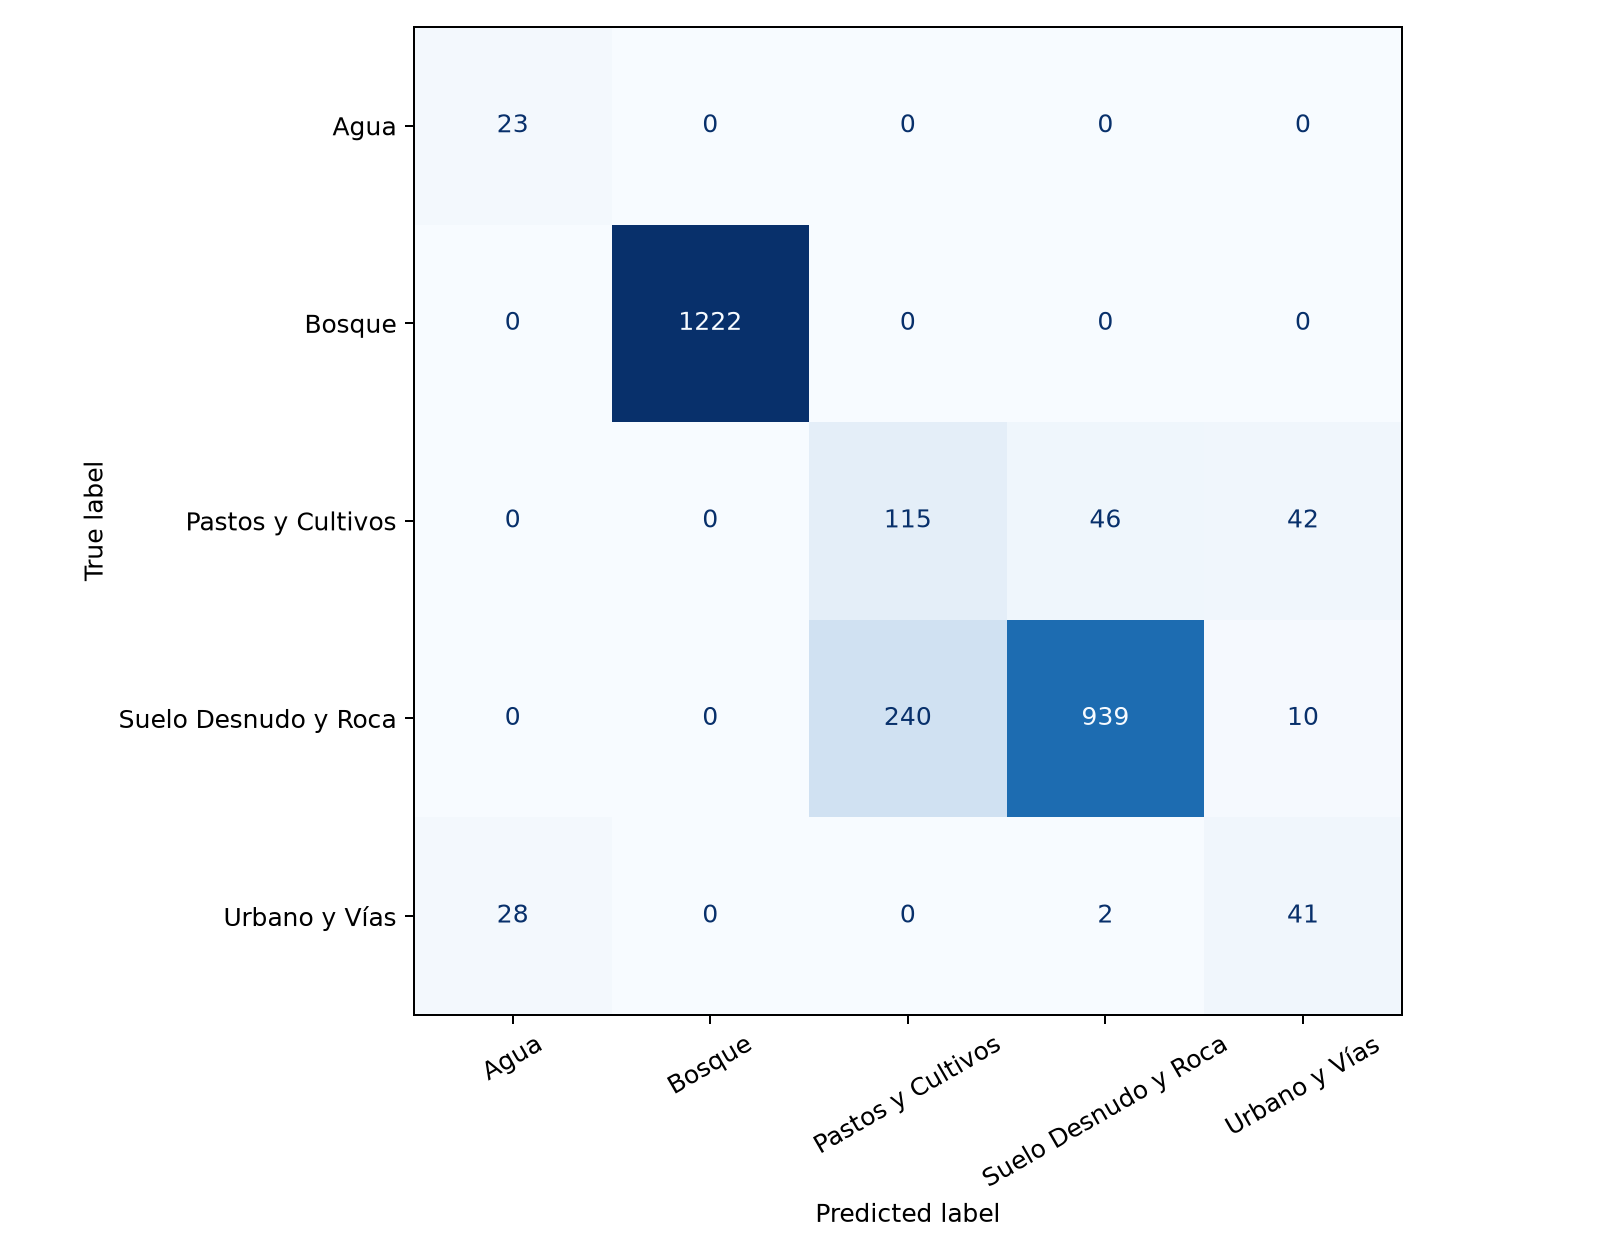
\includegraphics[width=\textwidth]{figures/decision_tree_confusion_matrix.png}
        \caption{Árbol de Decisión: 2.340/2.708.}
    \end{subfigure}
    \hfill
    \begin{subfigure}[b]{0.48\textwidth}
        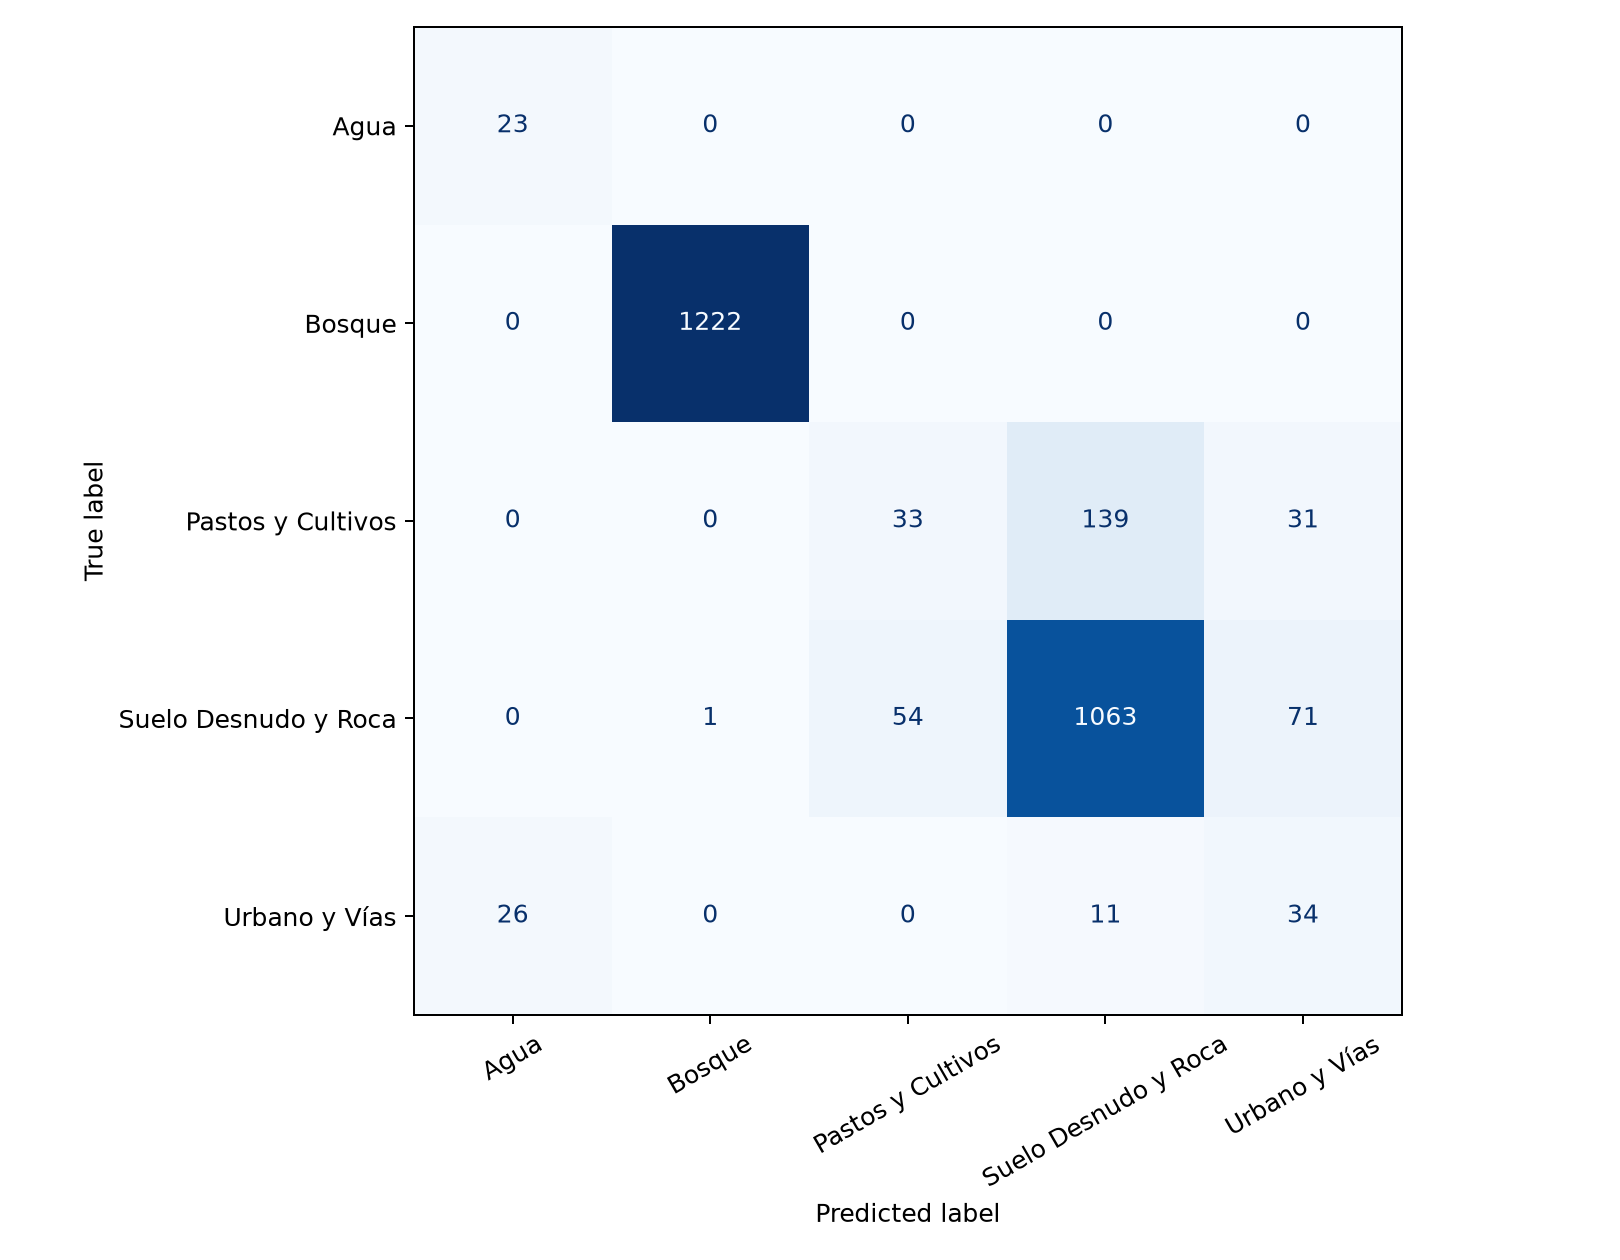
\includegraphics[width=\textwidth]{figures/knn_confusion_matrix.png}
        \caption{KNN ($k=15$): 2.375/2.708.}
    \end{subfigure}
    \caption{Matrices de confusión de los modelos evaluados sobre las 2.708 muestras del test independiente.}
    \label{fig:conf_matrices}
\end{figure}

\begin{itemize}[leftmargin=*,noitemsep,topsep=2pt]
    \item \textbf{Bosque (1.222 píxeles):} Separación perfecta en las cinco arquitecturas ($Recall = 1,0000$), sin ninguna omisión gracias a la alta reflectancia en \texttt{B08} y absorción en \texttt{B04}.
    \item \textbf{Suelo Desnudo y Roca (1.189 píxeles):} SVM RBF obtiene el mejor compromiso de frontera no lineal (1.067 aciertos, $F1 = 0,9023$), seguido por KNN (1.063) y ANN (1.024). Por el contrario, la Regresión Logística lineal desvía 299 píxeles de Suelo hacia Pastos y 75 hacia Urbano, castigando su recall a 68,38~\%.
    \item \textbf{Urbano y Vías (71 píxeles):} Representa la clase más exigente por mezcla espectral con suelo seco y techos metálicos/asfálticos. La \textbf{ANN/MLP} obtiene la mayor precisión (\textbf{62,50~\%}) y el mayor F1 (\textbf{0,5926}), con 24 falsos positivos urbanos frente a 66 en SVM, 101 en Regresión Logística y 102 en KNN. Como el test incluye un único polígono urbano, esta ventaja debe interpretarse con cautela.
    \item \textbf{Agua (23 píxeles):} Todos los clasificadores detectan los 23 píxeles del polígono de prueba de Agua ($Recall = 1,0000$), pero cometen entre 25 y 28 comisiones, todas provenientes de píxeles de referencia de Urbano y Vías.
\end{itemize}

\section{Inferencia ráster completa y cuantificación de áreas}

\subsection{Dominio de inferencia}
Para cumplir con la Sección 3.4 del enunciado~\cite{calderon2026}, se ejecutó la predicción sobre el cubo multiespectral completo en \texttt{EPSG:9377}. Si bien la máscara general (\texttt{mask\_valid.tif}) delimita 471.579 celdas libres de nubes en el visible, las bandas \textit{Red Edge} y NIR estrecho (\texttt{B05}, \texttt{B06}, \texttt{B07}, \texttt{B8A}) presentan bordes con \texttt{NoData} en los márgenes de la adquisición. Para no imputar reflectancias, la inferencia oficial (\texttt{src/predict\_raster\_hania.py}) clasificó solo los píxeles con máscara válida y valores finitos, positivos y distintos de NoData en las diez bandas, es decir, la \textbf{intersección física estricta de las diez bandas: exactamente 342.525 píxeles válidos (3.425,25~ha = 34,2525~$\text{km}^2$)}.

Fuera de ese dominio, el GeoTIFF de salida conserva el valor 0 (NoData). Cada salida es un ráster \texttt{uint8} de una banda con códigos 1 a 5, el mismo CRS y la misma transformación afín del stack. La Tabla~\ref{tab:areas_ann} presenta las superficies obtenidas con ANN. \estadoauditoria

\begin{table}[H]
\centering
\small
\resizebox{\textwidth}{!}{\begin{tabular}{c l c r r r r}
\toprule
\textbf{Class\_ID} & \textbf{Cobertura terrestre} & \textbf{Color QGIS} & \textbf{Píxeles} & \textbf{Área (ha)} & \textbf{Área ($\text{km}^2$)} & \textbf{Superficie (\%)} \\
\midrule
1 & \textbf{Bosque}                  & \texttt{\#1b7837} (Verde)   & 218.951 & 2.189,51 & 21,8951 & 63,92\,\% \\
3 & \textbf{Suelo Desnudo y Roca}    & \texttt{\#d73027} (Rojo)    & 117.213 & 1.172,13 & 11,7213 & 34,22\,\% \\
2 & \textbf{Pastos y Cultivos}       & \texttt{\#a6d96a} (Pastel)  & 3.822   & 38,22    & 0,3822  & 1,12\,\%  \\
4 & \textbf{Urbano y Vías}           & \texttt{\#e08214} (Naranja) & 1.993   & 19,93    & 0,1993  & 0,58\,\%  \\
5 & \textbf{Agua}                    & \texttt{\#2166ac} (Azul)    & 546     & 5,46     & 0,0546  & 0,16\,\%  \\
\midrule
— & \textbf{Total analizado (10 bandas)} & —                       & \textbf{342.525} & \textbf{3.425,25} & \textbf{34,2525} & \textbf{100,00\,\%} \\
\bottomrule
\end{tabular}}
\caption{Superficie por cobertura obtenida con la Red Neuronal Artificial (ANN/MLP), según \texttt{outputs/metrics/inferencia\_10bandas/area\_stats\_ann.json}.}
\label{tab:areas_ann}
\end{table}

\subsection{Sensibilidad espacial entre las cinco arquitecturas}
La Tabla~\ref{tab:sensibilidad_areas} compara la distribución superficial predicha por los cinco modelos sobre el dominio canónico de 342.525 píxeles:

\begin{table}[H]
\centering
\small
\resizebox{\textwidth}{!}{\begin{tabular}{l r r r r r}
\toprule
\textbf{Cobertura terrestre} & \textbf{ANN / MLP (ha)} & \textbf{SVM RBF (ha)} & \textbf{KNN (ha)} & \textbf{Árbol CART (ha)} & \textbf{Reg. Logística (ha)} \\
\midrule
Bosque                  & 2.189,51 (63,9\,\%) & 2.180,01 (63,6\,\%) & 2.223,36 (64,9\,\%) & 1.544,52 (45,1\,\%) & 2.521,82 (73,6\,\%) \\
Suelo Desnudo / Roca    & 1.172,13 (34,2\,\%) & 1.180,54 (34,5\,\%) & 1.148,70 (33,5\,\%) & 1.768,50 (51,6\,\%) & 616,46 (18,0\,\%)   \\
Pastos y Cultivos       & 38,22 (1,1\,\%)     & 37,26 (1,1\,\%)     & 23,92 (0,7\,\%)     & 80,48 (2,4\,\%)     & 254,97 (7,4\,\%)    \\
Urbano y Vías           & 19,93 (0,6\,\%)     & 22,23 (0,6\,\%)     & 22,95 (0,7\,\%)     & 25,70 (0,8\,\%)     & 25,98 (0,8\,\%)     \\
Agua                    & 5,46 (0,2\,\%)      & 5,21 (0,2\,\%)      & 6,32 (0,2\,\%)      & 6,05 (0,2\,\%)      & 6,02 (0,2\,\%)      \\
\midrule
\textbf{Total escena}   & \textbf{3.425,25 ha} & \textbf{3.425,25 ha} & \textbf{3.425,25 ha} & \textbf{3.425,25 ha} & \textbf{3.425,25 ha} \\
\bottomrule
\end{tabular}}
\caption{Sensibilidad y concordancia de áreas clasificadas entre las cinco arquitecturas sobre el dominio común.}
\label{tab:sensibilidad_areas}
\end{table}

ANN y SVM presentan resultados próximos en Bosque (diferencia de 9,50~ha) y en Suelo Desnudo y Roca (8,41~ha). KNN difiere de ANN en 33,85~ha de Bosque y 23,43~ha de Suelo Desnudo y Roca, por lo que no corresponde afirmar una convergencia uniforme. El Árbol de Decisión y la Regresión Logística se apartan mucho más: la Regresión Logística asigna 616,46~ha a Suelo Desnudo y Roca (18,0~\%) y 254,97~ha a Pastos y Cultivos (7,4~\%), en coherencia con la confusión Suelo$\rightarrow$Pastos observada en su matriz. La superficie cartografiada depende, por tanto, del clasificador elegido.

\subsection{Cartografía temática en QGIS}
El archivo GeoTIFF \texttt{landcover\_ann.tif} se importó en QGIS~3.44.13 (\nolinkurl{outputs/rasters/Clasificacion_Cobertura_ANN.qgz}), aplicando la paleta categórica oficial \texttt{landcover\_style.qml}. La composición cartográfica final (Figura~\ref{fig:mapa_qgis}) incluye leyenda de las cinco clases, escala gráfica, norte, cuadro de áreas y referencia \texttt{EPSG:9377}. Las zonas en blanco corresponden a píxeles sin clasificar (NoData en alguna de las diez bandas).

\begin{figure}[H]
    \centering
    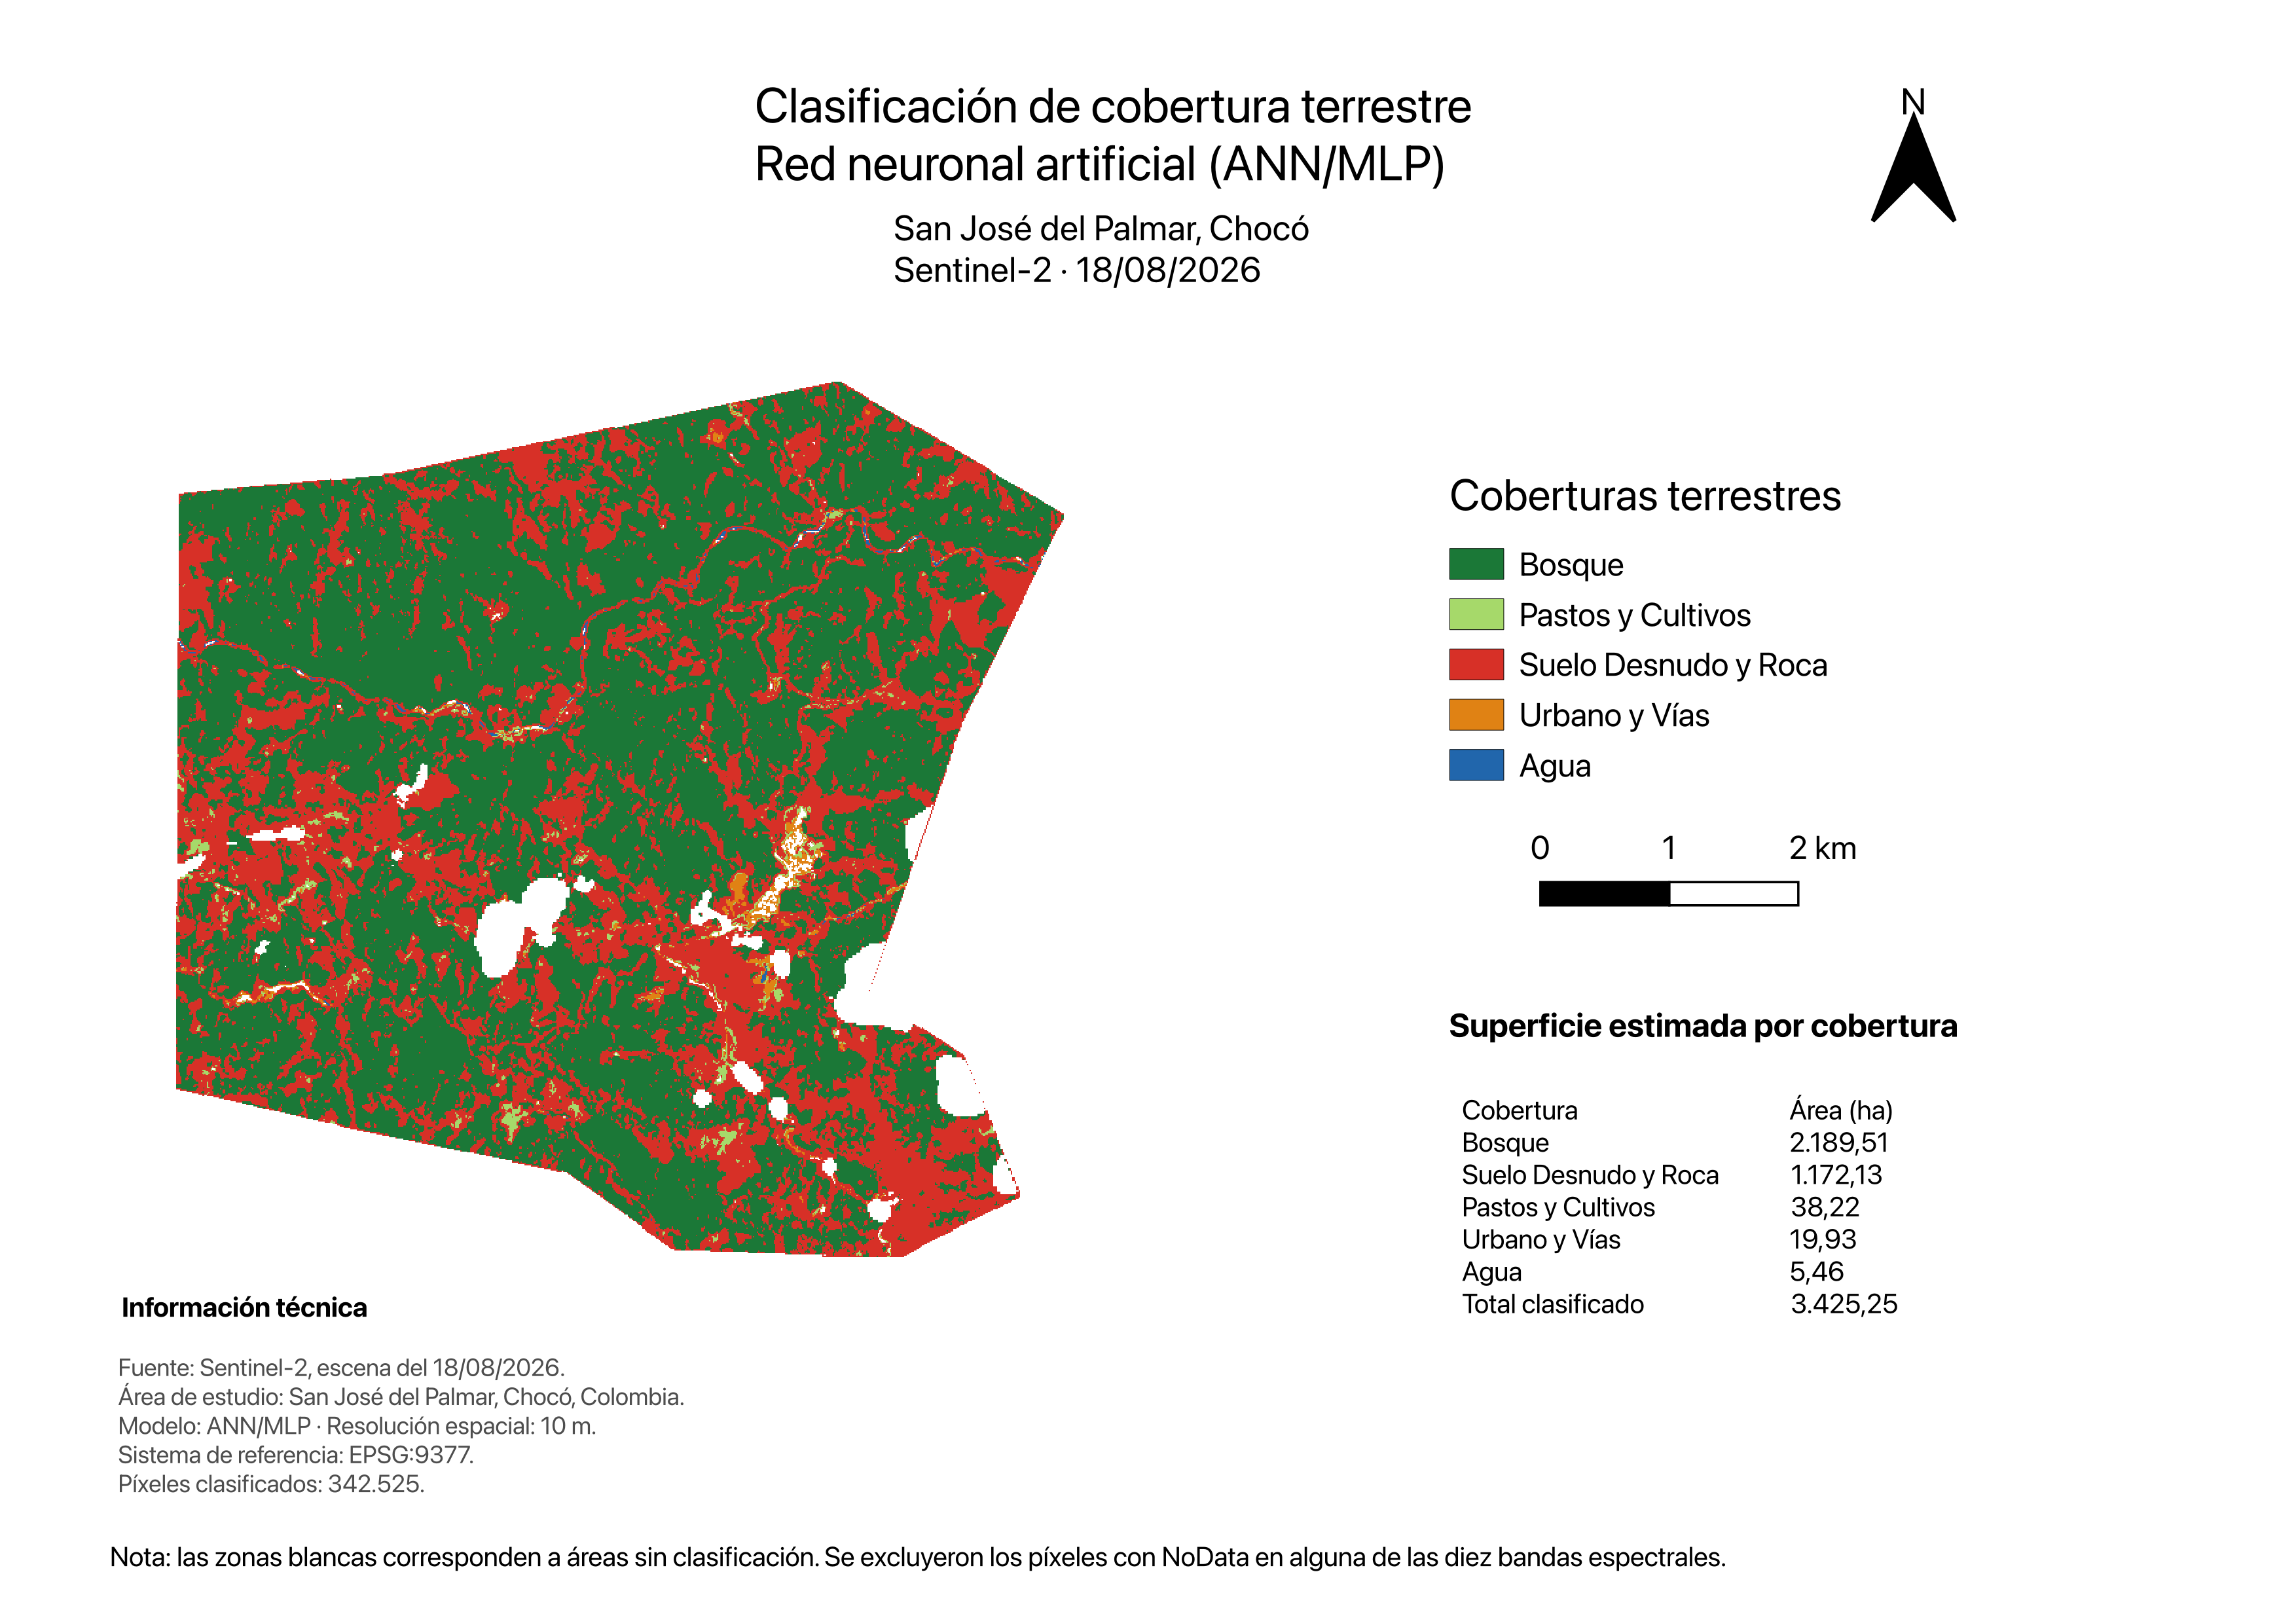
\includegraphics[width=0.95\textwidth]{figures/mapa_ann.png}
    \caption{Mapa temático oficial de coberturas terrestres post-sismo en San José del Palmar (Chocó) obtenido con la Red Neuronal Artificial (ANN/MLP) en QGIS. El cuadro de áreas reproduce los valores de \texttt{area\_stats\_ann.json}.}
    \label{fig:mapa_qgis}
\end{figure}

\section{Limitaciones}
\label{sec:limitaciones}
\begin{itemize}[leftmargin=*,noitemsep,topsep=2pt]
    \item \textbf{Pocos polígonos de prueba en clases minoritarias:} Agua y Urbano y Vías tienen un único polígono de prueba, y Pastos y Cultivos dos. Sus métricas por clase son frágiles y las diferencias entre modelos en esas clases no son generalizables.
    \item \textbf{Sin pruebas de significancia:} no se aplicaron pruebas estadísticas (por ejemplo, McNemar) entre modelos; las diferencias de desempeño se reportan como descriptivas.
    \item \textbf{Una sola escena:} sin una imagen previa al sismo no es posible separar el suelo expuesto por el evento del preexistente.
    \item \textbf{Cobertura de la inferencia:} se clasificó el 72,6~\% de las celdas de la máscara (342.525 de 471.579). Las 129.054 restantes tienen NoData en al menos una banda, concentrado en \texttt{B05}, \texttt{B06}, \texttt{B07} y \texttt{B8A}.
    \item \textbf{Polígonos sin muestras:} 95 de los 240 polígonos digitalizados no aportaron píxeles; su causa individual (fuera de la escena, fuera de la máscara o NoData en alguna banda) está pendiente de verificación.
    \item \textbf{Optimización acotada:} las grillas de hiperparámetros son pequeñas (50 combinaciones en total) y no se evaluaron ensambles como Random Forest o Boosting.
    \item \textbf{Versión de serialización:} \texttt{models/logistic\_regression.joblib} fue serializado con scikit-learn~1.9.1; en el entorno de referencia (1.5.2) emite una advertencia de versión, aunque sus métricas de prueba se reproducen exactamente.
\end{itemize}

\section{Reproducibilidad y entregables}
El código fuente, los modelos serializados, las particiones y las métricas se encuentran en el repositorio del proyecto~\cite{repo2026}. El entorno de referencia es Python~3.12.10 con numpy~1.26.4, scikit-learn~1.5.2 y rasterio~1.4.4 (\texttt{requirements.txt}). Las métricas de prueba de los cinco modelos se recalcularon desde los archivos \texttt{.joblib} y coinciden exactamente con las reportadas en la Tabla~\ref{tab:comparacion_modelos}; la suite de pruebas automáticas (\texttt{pytest}, 8 pruebas) se ejecuta sin errores. El flujo de inferencia y auditoría se documenta en \texttt{README.md} y \texttt{docs/DECISIONES\_INFERENCIA.md}. Los entregables son: (i) el GeoTIFF temático \texttt{landcover\_ann.tif}; (ii) este informe técnico, y (iii) el código fuente en ZIP.

\section{Discusión y conclusiones}

\begin{enumerate}[leftmargin=*,noitemsep,topsep=2pt]
    \item \textbf{Cumplimiento del flujo GeoAI:} Se completó el ciclo desde la preparación de Sentinel-2 L2A en \texttt{EPSG:9377} hasta el TSV de diez bandas y 14.155 muestras, la optimización con validación cruzada agrupada por polígono, la evaluación de cinco modelos sobre el mismo conjunto de prueba reservado y la inferencia ráster con cuantificación de superficies.
    \item \textbf{Selección del modelo:} SVM RBF obtuvo el mayor Overall Accuracy (89,70~\%) y Kappa (0,8283); la ANN/MLP, el mayor Macro-F1 (0,7075 en test y 0,7103 en validación cruzada). Se eligió ANN para el mapa temático porque Macro-F1 fue la métrica priorizada desde la optimización para equilibrar las cinco clases. ANN no supera a SVM en todas las clases: empatan en Agua y Bosque, ANN mejora Urbano y Vías (precisión 62,50~\% frente a 39,45~\%, 23,05 puntos porcentuales) y SVM mejora ligeramente Pastos y Suelo Desnudo. SVM queda como alternativa documentada.
    \item \textbf{Contribución espectral:} en el árbol de decisión, \texttt{B08} y \texttt{B04} concentraron el 66,48~\% de la importancia Gini, y \texttt{B02}, \texttt{B11} y \texttt{B05} también aportaron. Estas importancias describen el uso de las bandas en ese árbol, pero no demuestran que cada banda sea indispensable.
    \item \textbf{Interpretación territorial:} la ANN clasificó 1.172,13~ha como Suelo Desnudo y Roca (34,22~\% de la superficie válida analizada). Es una predicción espectral sobre una escena posterior al sismo, no una observación de campo; atribuir esas hectáreas al evento requiere una comparación bitemporal y evidencia adicional.
    \item \textbf{Trabajo futuro:} incorporar una escena previa al evento para análisis de cambio, aumentar los polígonos independientes de las clases minoritarias, evaluar ensambles (Random Forest, Boosting) y aplicar pruebas de significancia entre modelos.
\end{enumerate}

\begin{thebibliography}{9}
\small
\bibitem{sgc2026}
Servicio Geológico Colombiano (SGC). \textit{Boletín actualizado sobre el sismo de San José del Palmar, Chocó ($M_w$ 7,4 del 10 de agosto de 2026)}. Bogotá D.C., 2026. Disponible en: \url{https://www.sgc.gov.co}.
\bibitem{calderon2026}
Calderón Romero, A. O. \textit{Final Project: A Comparative Analysis of Machine Learning Architectures for Satellite-Based Land Cover Classification}. Guía de curso, Pontificia Universidad Javeriana, 2026.
\bibitem{lillesand2015}
Lillesand, T., Kiefer, R. W., y Chipman, J. \textit{Remote Sensing and Image Interpretation}. 7ma ed., John Wiley \& Sons, 2015.
\bibitem{roberts2017}
Roberts, D. R., et al. Cross-validation strategies for data with temporal, spatial, hierarchical, or phylogenetic structure. \textit{Ecography}, 40(8):913--929, 2017.
\bibitem{congalton2019}
Congalton, R. G., y Green, K. \textit{Assessing the Accuracy of Remotely Sensed Data: Principles and Practices}. 3ra ed., CRC Press, 2019.
\bibitem{pedregosa2011}
Pedregosa, F., et al. Scikit-learn: Machine Learning in Python. \textit{Journal of Machine Learning Research}, 12:2825--2830, 2011.
\bibitem{repo2026}
León, N., Barrios, A., Carreño, H., y Sierra, J. \textit{Repositorio EmergentesFinal: Flujo GeoAI reproducible}. Código fuente, particiones y modelos serializados. GitHub, 2026. \url{https://github.com/Nicolas11Leon/EmergentesFinal}.
\end{thebibliography}

\end{document}
